\documentclass [a4paper,12pt]{article}
\usepackage{amsmath,amsthm,amssymb}
\usepackage{graphicx}
\usepackage{mathtext}
\usepackage[T1,T2A]{fontenc}
\usepackage[utf8]{inputenc}
\usepackage[english,russian]{babel}
\usepackage{tikz}


\title{Домашние задание №3 по дисциплине "Теория случайных процессов"}

\author{Головатских Марк \\БПМ-16-1 \\ Вариант 6}
\date{}
\begin{document}

\maketitle
\pagenumbering{gobble}
\newpage
\pagenumbering{arabic}
Построим граф состояний, где каждое состояние процесса - число сломанных приборов.\\
\begin{figure}[h!]
  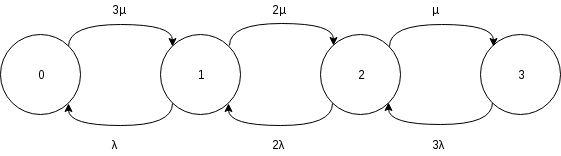
\includegraphics[width=\linewidth]{pic3.png}
\end{figure}\\
Составим уравнения Колмогорова:\\
\begin{equation*}
\begin{cases}
  P'_0(t) = -3{\mu}P_0(t) + {\lambda}P_1(t)
  \\
  P'_1(t) = 3{\mu}P_0(t) + 2{\lambda}P_2(t) - (\lambda + 2{\mu})P_1(t)
  \\
  P'_2(t) = 2{\mu}P_1(t) + 3{\lambda}P_3(t) - (2{\lambda} + \mu)P_2(t)
  \\
  P'_3(t) = - 3{\lambda}P_2(t) + {\mu}P_3(t)
\end{cases}
\end{equation*}
Из записи этой системы в матричной форме получим инфинитезимальную матрицу:\\
$A = \left(
\begin{matrix}
-3{\mu} & 3{\mu} & 0 & 0\\
\lambda & -({\lambda} + 2{\mu}) & 2{\mu} & 0\\
0 & 2{\lambda} & -(2{\lambda} + \mu) & \mu \\
0 & 0 & 3{\lambda} & -3{\lambda} \\
\end{matrix}
\right) $\\
Из условий $\mu = \lambda = 3$. Составим систему для нахождения финальных вероятностей:\\
\begin{equation*}
\begin{cases}
0 = 3p_1 - 9p_0
\\
0 = 6p_2 + 9p_0 - 9p_1
\\
0 = 6p_1 + 9p_3 - 9p_2
\\
0 = 3p_2 - 9p_3
\end{cases}
\end{equation*}
Учитывая соотношение $p_0 + p_1 + p_2 + p_3 = 1$, заменим на него одно из уравнений:
\begin{equation*}
\begin{cases}
0 = 3p_1 - 9p_0
\\
0 = 9p_2 + 6p_0 - 9p_1
\\
0 = 6p_1 + + 9p_3 - 9p_2
\\
p_0 + p_1 + p_2 + p_3 = 1
\end{cases}
\end{equation*}
Решение:
\begin{equation*}
\begin{cases}
p_0 = \frac{1}{8}
\\
p_1 = \frac{3}{8}
\\
p_2 = \frac{3}{8}
\\
p_3 = \frac{1}{8}
\end{cases}
\end{equation*}
Для нахождения зависимости среднего состояния от времени найдем математическое ожидание числа сломанных приборов.\\
$\lambda_i = i{\lambda}$, $\mu_i = (n-i){\mu}$. С учетом начальных условий получим:\\
\begin{equation*}
\begin{cases}
MX'(t) = (\lambda + \mu)MX(t) - {\mu}N
\\
MX(0) = 3
\\
\end{cases}
\end{equation*}
Решением является $MX(t) = \frac{1}{3}e^{6t}+\frac{3}{2}$.
\end{document}
